\documentclass[handout]{beamer}
%\documentclass{article}
\usepackage{animate}
\usepackage{array}
\newcommand{\degC}[1]{\ensuremath{#1\,^{\circ}\mathrm{C}}}
\setbeamertemplate{navigation symbols}{}
\setbeamertemplate{caption}{\insertcaption} \setbeamertemplate{caption label separator}{}
\renewcommand{\emph}{\textbf}
\usetheme{Warsaw}
\title{Ch. 4 -- Continuous Random Variables}
%\setlength{\parskip}{.2cm}
\DeclareMathOperator{\Bin}{Bin}

\begin{document}
\begin{frame}
\begin{beamercolorbox}[rounded=true,wd=\textwidth,center]{title}
\usebeamerfont{title}\inserttitle
\end{beamercolorbox}
\begin{center}
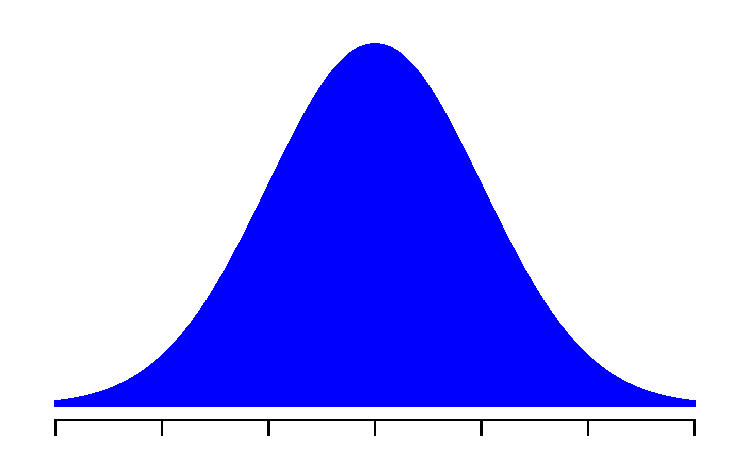
\includegraphics[scale=.7]{ch4_cdf_norm3.pdf}
\end{center}
\end{frame} 

%\begin{frame}{Probability Measures}
%Recall that given a set $\Omega$ of outcomes, subsets of $\Omega$ are called \emph{events}, and a \emph{probability measure} on $\Omega$ is a function which assigns a number $P(A)$ to events $A$, such that
%\begin{enumerate}
%\item $P(A)\geq 0$ for all events $A$.
%\item $P(\Omega)=1$.
%\item If $A_1,A_2,\dots$ are disjoint events, then
%$$P(A_1\cup A_2\cup \cdots)=\sum_{i=1}^\infty P(A_i)$$
%\end{enumerate}
%\end{frame}
%
%\begin{frame}{Simple events}
%A \emph{simple event} is an event containing only one outcome. If an event $A$ contains only the outcome $a$, then we write $A=\{a\}$. If the outcomes in an event $A$ can be written in a sequence $a_1, a_2, a_3, \dots$, then its probability is simply the sum of the probabilities of the simple events it contains:
%\begin{align*}
%P(A)&=P(\{a_1,a_2,a_3,\dots\})\\
%&=P(\{a_1\} \cup \{a_2\} \cup \{a_3\}\cup \cdots) \\
%&= P(\{a_1\}) + P(\{a_2\}) + P(\{a_3\}) + \cdots +
%\end{align*}
%\pause In particular, if the outcomes in $\Omega$ can be written in a sequence, then the probability of any event can be found by just adding up the probabilities of simple events.
%
%\pause\vspace{.2cm} \textit{Caution}: This does not work if the set of outcomes in an event is too large to be written in a sequence.
%\end{frame}

\begin{frame}{Continuous Random Variables}
So far, we have only discussed discrete random variables, which have only a sequence of possible values (usually whole numbers):
\begin{itemize}
\item The number of defective widgets in a batch.
\item The number of widgets inspected before finding one defective.
\item The number of customers who visit a store in an hour.
\end{itemize}
However, many quantities in real life vary continuously:
\begin{itemize}
\item The length of a metal rod.
\item The strength of a specimen of concrete.
\item The weight of a bottled drink.
\item The amount of time until the next customer arrives.
\end{itemize}
We will need different techniques to deal with continuous random variables.
\end{frame}

\begin{frame}{Uniform Random Variable}
\begin{block}{}
Suppose we choose a random number $X$ ``uniformly" from the interval $[0,1]$. 
What is the probability that we get a number between 0.2 and 0.6?
\end{block}
\pause \begin{figure}[H]
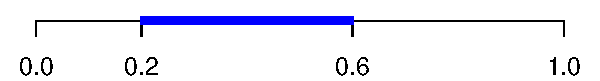
\includegraphics{ch4_interval.pdf}
\end{figure}
\pause The interval $[0.2, 0.6]$ has length $0.6-0.2=0.4$, which is 40\% of the total length of the interval $[0,1]$. Therefore, intuitively the probability that $X$ would be in the interval $[0.2, 0.6]$ should be
$$ P(0.2 \leq X \leq 0.6) = 0.6-0.2 = 0.4$$
In general, for an interval $[a,b]$ inside $[0,1]$ we should have
$$ P(a \leq X \leq b) = b- a$$
\end{frame}

\begin{frame}{Uniform Random Variable}
\begin{block}{}
Suppose we choose a random number from the interval $[0,1]$. What is the probability that we get exactly the number 0.5?
\end{block}
\pause \begin{figure}[H]
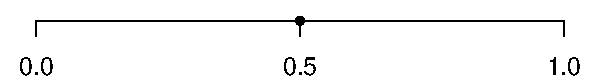
\includegraphics{ch4_interval2.pdf}
\end{figure}
\pause
The probability is 
$P(0.5 \leq X \leq 0.5) = 0.5 - 0.5 = 0$. In fact, for any $x$ in $[0,1]$ the probability that $X$ is exactly $x$ is 0. And yet, $X$ will always be some number in $[0,1]$. %This may seem like a paradox, but what it means is this:

\begin{itemize}
\pause \item Even if an event has probability 0, that doesn't mean it is impossible for it to occur.
\pause \item For a continuous random variable, the concept of a probability mass function is useless: every probability $P(X=x)$ is zero. 
\pause \item We \textit{cannot} find the probability $P(a \leq X \leq b)$ by simply adding up all the probabilities $P(X=x)$ over all $x$ in $[a,b]$.
\end{itemize}
\end{frame}

\begin{frame}{Continuous Random Variable}
\begin{block}{}
We say that a random variable $X$ is \emph{continuous} if $P(X=x)=0$ for every $x$. If there is a function $f(x)$ such that for all $a\leq b$,
$$P(a \leq X \leq b) = \int_a^b f(x)\ dx$$
then we call $f(x)$ a \emph{probability density function} (pdf) of $X$.
\end{block}


\begin{tabular}{p{5cm}p{4.5cm}}
\vspace{.4cm} To be a valid pdf, we must have
\begin{enumerate}
\item $f(x)\geq 0$ for all $x$.
\item $\int_{-\infty}^{\infty} f(x)=1$.
\end{enumerate}
&
\vspace{-.55cm}
\hspace*{-.6cm}
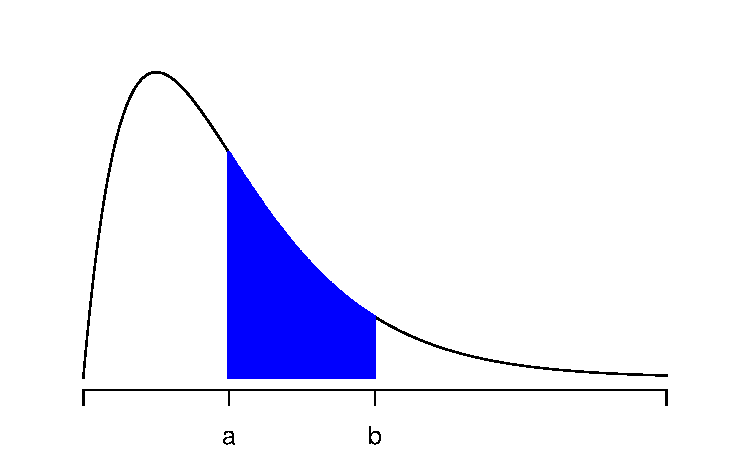
\includegraphics[scale=.55]{ch4_pdf_gam.pdf}
\end{tabular}
\end{frame}

\begin{frame}{Standard Uniform Random Variable}
Define a pdf by
$$f(x)=\begin{cases}1 & \text{if }0\leq x\leq 1 \\
0 & \text{otherwise}\end{cases}$$
The continuous random variable $X$ with this pdf is called a \emph{standard uniform} random variable; it takes values uniformly on the interval [0,1].
\begin{tabular}{@{}p{5.5cm}p{4.5cm}}
\vspace{0cm}For example, the probability that $X$ is between .2 and .6 is
\begin{center}$\begin{aligned}[t]
&P(.2 \leq X \leq .6) \\
&=\int_{.2}^{.6} 1\ dx\\
&= x\vert_{.2}^{.6}\\
&= .6-.2\\
&=.4
\end{aligned}$\end{center}
&
\vspace{0cm}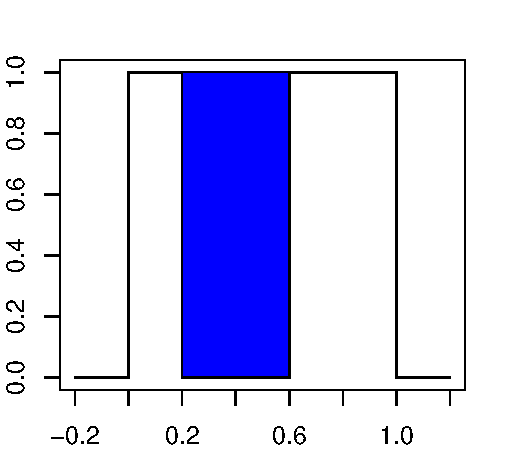
\includegraphics[scale=.6]{ch4_pdf_unif.pdf}
\end{tabular}
\end{frame}

\begin{frame}{Uniform Random Variable}
\begin{block}{}
We say that $X$ is a \emph{uniform} random variable on the interval $[a,b]$ if $X$ has pdf
$$f(x)=\begin{cases}\frac1{b-a} & \text{if }a\leq x\leq b \\
0 & \text{otherwise}\end{cases}$$
\end{block}
\pause Example: Suppose that the time we have to wait at a bus stop is a uniform random variable $X$ between 0 and 15 minutes. What is the probability that we will have to wait more than 10 minutes?
\pause \begin{align*}
P(X\geq 10) &= \int_{10}^\infty f(x)\ dx \\
&= \int_{10}^{15} \frac1{15-0}\ dx \\
&= \frac1{15}x\big\vert_{10}^{15} \\
&= \frac{15-10}{15} = 1/3
\end{align*}
\end{frame}



\begin{frame}{Exponential Random Variable}
\begin{block}{}
We say that $X$ is an \emph{exponential} random variable with rate $\lambda>0$ if $X$ has pdf
$$f(x) = \begin{cases}\lambda e^{-\lambda x} & \text{if }x\geq 0 \\ 0 & \text{if }x<0\end{cases}$$
\end{block}
\pause We can check that this is a valid pdf:

\begin{tabular}{p{5.5cm}p{4cm}}
\vspace{0cm}
$\begin{aligned}[t]
\int_{-\infty}^\infty f(x)\ dx &= \int_0^\infty \lambda e^{-\lambda x}\ dx \\
&= \lambda \frac{-1}\lambda e^{-\lambda x}\Big\vert_{x=0}^\infty\\
&= 0 - (-1) = 1
\end{aligned}$
&
\vspace{-.25cm}
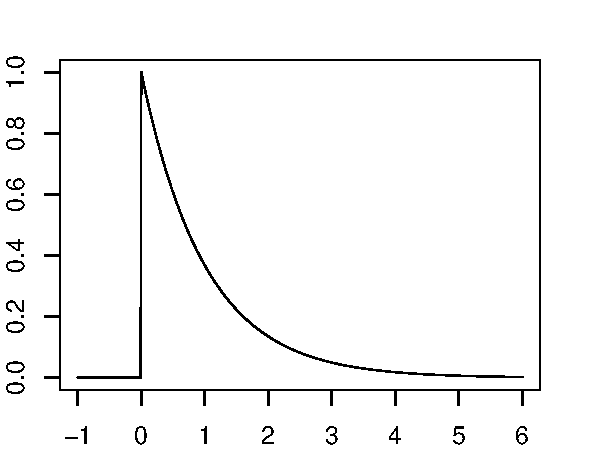
\includegraphics[scale=.55]{ch4_pdf_exp.pdf}
\end{tabular}
\end{frame}

\begin{frame}{CDF of Continuous Random Variable}
The \emph{cumulative distribution function} (cdf), $F(x)$, of a continuous random variable $X$ is defined the same as in the discrete case:
$$F(x) = P(X \leq x)$$
\pause If $X$ has pdf $f(x)$, then this becomes
$$F(x) = \int_{-\infty}^x f(t)\ dt$$
\pause By the Fundamental Theorem of Calculus, $F'(x)=f(x)$, if $f$ is continuous at $x$ .
\vspace{-.5cm}
\begin{center}
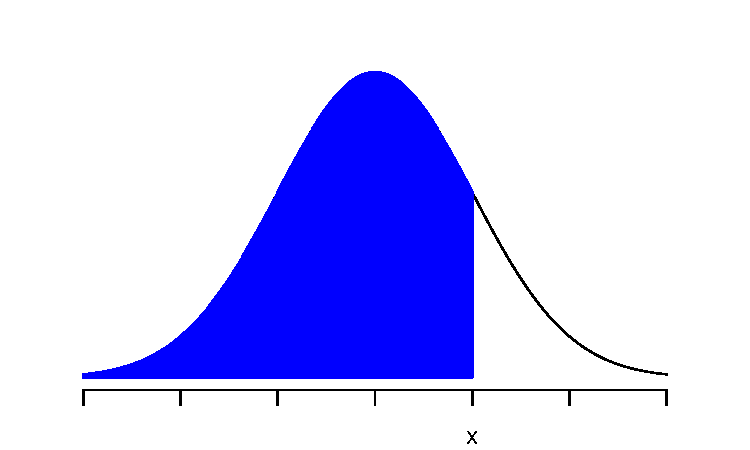
\includegraphics[scale=.5]{ch4_cdf_norm.pdf}
\end{center}
\end{frame}

\begin{frame}{CDF of Standard Uniform Random Variable}
Recall that a standard uniform random variable $X$ has pdf
$$f(x)=\begin{cases}1 & \text{if }0\leq x\leq 1 \\
0 & \text{otherwise}\end{cases}$$

\pause Let $F(x)$ be the cdf of $X$. For $0\leq x\leq 1$, we have
$$F(x)=\int_{-\infty}^x f(t)\ dt = \int_0^x 1\ dt = x$$

\pause For $x\leq0$, clearly $F(x)=0$, while for $x\geq 1$, $F(x)=1$.

\vspace{-1.2cm}
\begin{center}
\begin{tabular}{@{}p{6cm}p{5cm}}
\vspace{0cm}
\centering 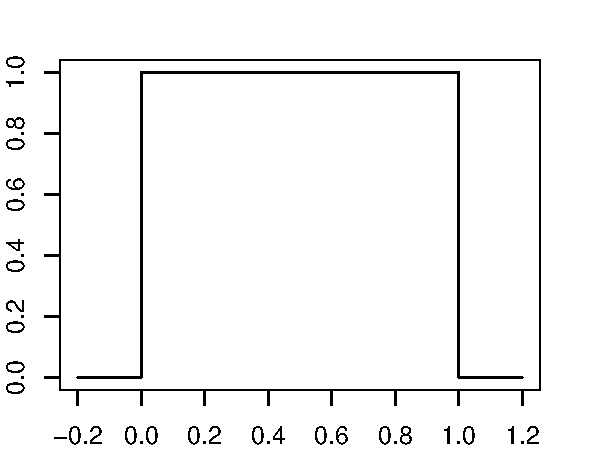
\includegraphics[scale=.5]{ch4_pdf_unif2.pdf}
&
\vspace{0cm}
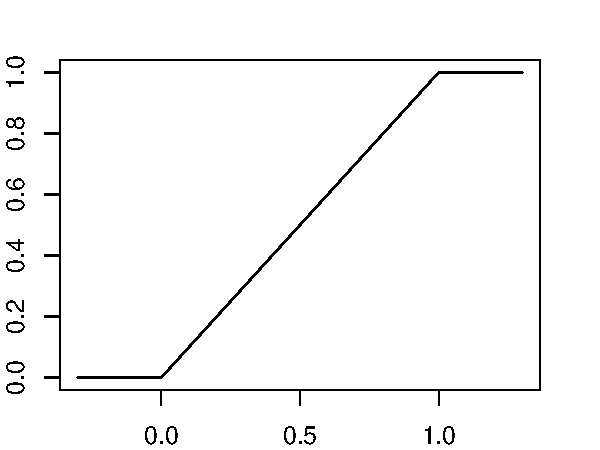
\includegraphics[scale=.5]{ch4_cdf_unif.pdf}\\
\centering $f(x)=\text{pdf of $X$}$ & \centering $F(x)=\text{cdf of $X$}$
\end{tabular}
\end{center}
\end{frame}

\begin{frame}{CDF of Exponential Random Variable}
Recall the pdf of an exponential random variable $x$ with rate $\lambda$ is 
$$f(x) = \begin{cases}\lambda e^{-\lambda x} & \text{if }x\geq 0 \\ 0 & \text{if }x<0\end{cases}$$
\pause The cdf $F(x)$ is therefore, for $x\geq 0$,
\begin{align*}
F(x)&=\int_{-\infty}^x f(t)\ dt=\int_0^x \lambda e^{-\lambda t}\ dt \\
&= -e^{-\lambda t}\big\vert_{t=0}^x = 1-e^{-\lambda x}
\end{align*}

\pause\newcolumntype{C}{>{\centering}p{5.5cm}} 
\begin{tabular}{CC}
\vspace{-.8cm}
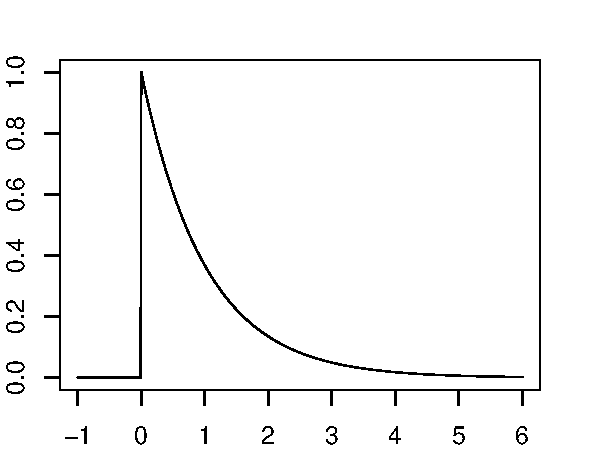
\includegraphics[scale=.5]{ch4_pdf_exp.pdf}
&
\vspace{-.8cm}
 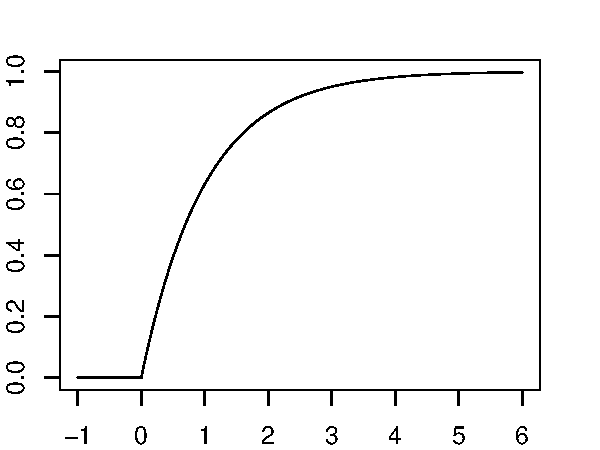
\includegraphics[scale=.5]{ch4_cdf_exp.pdf} \tabularnewline
 $f(x) = \text{pdf of $X$}$ & $F(x) = \text{cdf of $X$}$
\end{tabular}
\end{frame}

\begin{frame}{Expected Value}
\begin{block}{}
The \emph{expected value} or \emph{mean} of a continuous random variable $X$ with pdf $f(x)$ is
$$E(X) = \int_{-\infty}^\infty xf(x)\ dx$$
\end{block}
\pause For example, the mean of a uniform random variable $X$ on $[a,b]$ is
\begin{align*}
E(X) &= \int_{-\infty}^{\infty} xf(x)\ dx \\
\uncover<3->{&= \int_a^b \frac{x}{b-a}\ dx \\}
\uncover<4->{&= \frac{x^2}{2(b-a)}\Big\vert_a^b \\}
\uncover<5->{&= \frac{b^2-a^2}{2(b-a)}} 
\uncover<6->{= \frac{(b-a)(b+a)}{2(b-a)}}  \uncover<7->{= \frac{a+b}2}
\end{align*}
\end{frame}

\begin{frame}{Mean of Exponential}
Using integration by parts, we can find the mean of an exponential random variable $X$ of rate $\lambda$:
\begin{align*}
E(X)&=\int_{-\infty}^\infty xf(x)\ dx \\
\uncover<2->{&=\int_0^\infty x\lambda e^{-\lambda x}\ dx \\}
\uncover<3->{&= -xe^{-\lambda x}\big\vert_0^\infty + \int_0^\infty e^{-\lambda x}\ dx \\}
\uncover<4->{&= 0 - 0 - \frac1{\lambda}e^{-\lambda x}\big\vert_0^\infty = \frac 1\lambda}
\end{align*}

\end{frame}

\begin{frame}{Example}
\begin{block}{}
Suppose that the lifetime $X$ of a lightbulb follows an exponential distribution with mean $\mu=100$ days. What is the probability that the lifetime is at least 50 days?
\end{block}

\pause \vspace{.2cm}Solution: The rate of failure is $\lambda = 1/\mu = 1/100$ per day. Therefore,
\begin{align*}
P(X \geq 50) &= \int_{50}^{\infty} \lambda e^{-\lambda x}\ dx \\
\uncover<3->{&= -e^{-\lambda x}\big\vert_{50}^{\infty} \\}
\uncover<4->{&= e^{-50\lambda} \\}
\uncover<5->{&= e^{-50/100} = e^{-1/2} \approx .607}
\end{align*}

\pause \vspace{-.2cm}
\uncover<6->{\begin{block}{}
In general, if $X$ is an exponential random variable with rate $\lambda$,
$$P(X \geq t)=e^{-\lambda t}$$
\end{block}}
\end{frame}

\begin{frame}{Example}
\begin{block}{}
Again suppose that the lifetime $X$ of a lightbulb follows an exponential distribution with mean $\mu=100$ days. Given that the bulb has survived for 30 days, what is the probability that it will last for at least 50 more?
\end{block}
\vspace{-.2cm}\pause \begin{align*}
P(X\geq80 \mid X\geq 30) &= \frac{P(X\geq 80 \cap X\geq 30)}{P(X\geq 30)} \\
\uncover<3->{&= \frac{P(X\geq 80)}{P(X\geq 30)} \\}
\uncover<4->{&= \frac{e^{-80\lambda}}{e^{-30\lambda}} \\}
\uncover<5->{&= e^{-50\lambda} = e^{-50/100}=e^{-1/2} \approx .607}
\end{align*}
\uncover<6->{This is the same as the probability of a new bulb lasting 50 days, as we calculated on the previous slide.}
\end{frame}

\begin{frame}{Memoryless Property of Exponential}
The exponential distribution is useful for modeling the lifetime of components where breakdowns are the result of sudden, random failures rather than gradual deterioration. 

\vspace{.2cm}\pause In general, an exponential random has the ``memoryless" property:
\begin{block}{}
\vspace{-.2cm}$$P(X\geq s+t \mid X\geq s) = P(X\geq t)$$
\end{block}

\vspace{.25cm}
\pause Proof: $\begin{aligned}[t]
P(X\geq s+t\mid X\geq s) &= \frac{P(X\geq s+t \cap X\geq s)}{P(X\geq s)} \\
&= \frac{P(X\geq s+t)}{P(X\geq s)} \\
&= \frac{e^{-\lambda(s+t)}}{e^{-\lambda s}} \\
&= e^{-\lambda t} = P(X\geq t)
\end{aligned}$
\end{frame}


\begin{frame}{Exponential Waiting Times}
Consider a Poisson process with rate $\lambda$. 
\begin{itemize}
\item Let $Y_t$ be the number of events occurring in the interval $[0,t]$.
\pause \item So $Y_t$ is a Poisson random variable with mean $\lambda t$.
\pause \item Let $X$ be the time of the first event.
\end{itemize}
\begin{align*}
P(X \leq t) &= P(\text{first event occurs by time $t$}) \\
\uncover<4->{&= P(\text{at least one event occurs in the interval $[0,t]$})\\}
\uncover<5->{&= P(Y_t \geq 1) \\}
\uncover<6->{&= 1- P(Y_t = 0) \\}
\uncover<7->{&= 1 - \frac{e^{-\lambda t}(-\lambda t)^0}{0!} \\}
\uncover<8->{&= 1 - e^{-\lambda t}}
\end{align*}
\uncover<9->{This is the cdf of an exponential random variable of rate $\lambda$. Therefore, in a Poisson process, the waiting time for the first event is an exponential random variable with rate $\lambda$.}
\end{frame}

\begin{frame}{Variance and Standard Deviation}
The \emph{variance} of a continuous random variable $X$ with pdf $f(x)$ is
$$V(X) = E[(X-\mu)^2] = \int_{-\infty}^{\infty} (x^2-\mu)f(x)\ dx$$
\pause\vspace{.2cm}As before, the \emph{standard deviation} is $\sigma=\sqrt{V(X)}$. 

\pause\vspace{.2cm}The shortcut formula for the variance also works for continuous random variables:
$$V(X) = E(X^2)-[E(X)]^2$$
\end{frame}

\begin{frame}{Variance of Uniform Distribution}
\begin{align*}
E(X^2) &= \int_a^b \frac{x^2}{b-a}\ dx
\uncover<2->{= \frac{x^3}{3(b-a)}\Big\vert_a^b}
\uncover<3->{= \frac{b^3-a^3}{3(b-a)}\\}
\uncover<4->{&= \frac{(b-a)(a^2+ab+b^2)}{3(b-a)} }
\uncover<5->{= \frac{a^2+ab+b^2}3\\[.7cm]}
\uncover<6->{V(X) &= E(X^2)-[E(X)]^2 \\}
\uncover<7->{&= \frac{a^2+ab+b^2}3 - \left(\frac{a+b}2\right)^2 \\}
\uncover<8->{&= \frac{a^2+ab+b^2}3 - \frac{a^2+2ab+b^2}{4} \\}
\uncover<9->{&= \frac{a^2-2ab+b^2}{12} = \frac{(b-a)^2}{12}}
\end{align*}
\end{frame}

\begin{frame}{Variance of Exponential Distribution}
We can find the variance of an exponential random variable $X$ by using integration by parts twice:
\pause\begin{align*}
E(X^2)&=\int_0^\infty x^2\cdot\lambda e^{-\lambda x}\ dx \\
\uncover<3->{&= -x^2 e^{-\lambda x}\big\vert_0^\infty-\int_0^\infty -2xe^{-\lambda x}\ dx \\}
\uncover<4->{&= 2\int_0^\infty xe^{-\lambda x}\ dx \\}
\uncover<5->{&= 0-0+2\left[-\frac1\lambda xe^{-\lambda x}\big\vert_0^\infty - \int_0^\infty -\frac1\lambda e^{-\lambda x}\ dx \right] \\}
\uncover<6->{&= 2\left[0-0-\frac1{\lambda^2}e^{-\lambda x}\big\vert_0^\infty\right] = \frac2{\lambda^2}}
\end{align*}
\uncover<7->{So $V(X)=E(X^2)-[E(X)]^2 = \frac2{\lambda^2} - \left(\frac1\lambda\right)^2=\frac1{\lambda^2}$.
In other words, the standard deviation is $\sigma=1/\lambda=\mu$.}
\end{frame}

%\begin{frame}{Independence of Continuous Random Variables}
%Recall that we say discrete random variables $X$ and $Y$ are independent if
%$$P(X=a \cap Y=b) = P(X=a)P(Y=b)$$
%for all possible values $a$ of $X$ and $b$ of $Y$.
%
%\pause\vspace{.2cm}However, for continuous random variables, this definition is useless since both sides of the equation are automatically 0. 
%\pause\begin{block}{}
%We say that continuous random variables $X$ and $Y$ are \emph{independent} if
%$$P(a\leq X\leq b \cap c\leq Y\leq d) = P(a\leq X \leq b)P(c\leq Y\leq d)$$
%for all real numbers $a,b,c,d$.
%\end{block}{}
%\end{frame}

\begin{frame}{Properties of Expected Value and Variance}
The same properties of expected value and variance which we used for discrete random variables also work for continuous random variables:
\begin{block}{}
\begin{enumerate}
\item $E(c) = c$
\item $E(cX) = cE(X)$
\item $E(X+Y) = E(X)+E(Y)$
%\item If $X$ and $Y$ are independent, then $E(XY) = E(X)E(Y)$.
\end{enumerate}
\end{block}

\begin{block}{}
\begin{enumerate}
\item $V(c) = 0$
\item $V(cX) = c^2V(X)$
\item $V(X+c) = V(X)$
\item If $X$ and $Y$ are independent, $V(X+Y)=V(X)+V(Y)$.
\end{enumerate}
\end{block}
\end{frame}

\begin{frame}{Shifting and Scaling a Uniform Distribution}
Starting with a uniform random variable $X$ on $[a,b]$, if we add or multiply by a constant $c$, then we obtain a new uniform random variable:

\vspace{.2cm}Namely, $X+c$ is a uniform random variable on $[a+c,b+c]$, while $cX$ is a uniform random variable on $[ca,cb]$.

\vspace{.2cm}\pause
Starting from a standard uniform random variable $U$ on $[0,1]$, a uniform random variable $X$ on $[a,b]$ may be obtained by scaling and shifting:
$$X=(b-a)U+a$$

\vspace{0cm}
\begin{itemize}
\item First notice that $(b-a)U$ is uniform on $[0,b-a]$.
\item Therefore $(b-a)U+a$ is uniform on $[0+a,(b-a)+a]=[a,b]$.
\end{itemize}
\end{frame}

\begin{frame}{Variance of Uniform Distribution}
We can use properties of variance to more easily find the variance of a uniform random variable $X$ on $[a,b]$:

\pause\vspace{.2cm}First we find the variance of a standard uniform random variable $U$:
\begin{align*}
E(U^2) &= \int_{-\infty}^{\infty} x^2f(x)\ dx 
\uncover<3->{= \int_0^1 x^2\ dx }
\uncover<4->{= 1/3\\}
\uncover<5->{V(U) &= E(U^2)-[E(U)]^2 }
\uncover<6->{= 1/3-(1/2)^2 }
\uncover<7->{= 1/12}
\end{align*}
\uncover<8->{Now any uniform random variable $X$ on $[a,b]$ may be written in terms of a standard uniform random variable as $X=(b-a)U+a$.} 
\uncover<9->{Therefore,}
\begin{align*}
\uncover<9->{V(X)&=V((b-a)U+a) \\[.2cm]}
\uncover<10->{&= V((b-a)U) \\}
\uncover<11->{&= (b-a)^2V(U)}
\uncover<12->{=\frac{(b-a)^2}{12}}
\end{align*}
\end{frame}

\begin{frame}{Median of a Continuous Random Variable}
\begin{block}{}
Given a continuous random variable $X$, the \emph{median} of $X$ is the value $\tilde\mu$ such that $P(X \leq \tilde\mu)=\frac12$.
\end{block}
\pause Example: The median of a uniform random variable $X$ on $[a,b]$ is $\frac{a+b}2$, since
\begin{tabular}{p{6.5cm}p{5cm}}
\vspace{0cm}
$\begin{aligned}[t]
P(X \leq \frac{a+b}2) &= \int_a^{\frac{a+b}2} f(x)\ dx \\
\uncover<3->{&= \int_a^{\frac{a+b}2} \frac1{b-a}\ dx \\}
\uncover<4->{&= \frac1{b-a}\left(\frac{a+b}2-a\right) \\}
\uncover<5->{&= \frac1{b-a}\cdot \frac{b-a}2 = \frac12}
\end{aligned}$
&
\vspace{0cm}
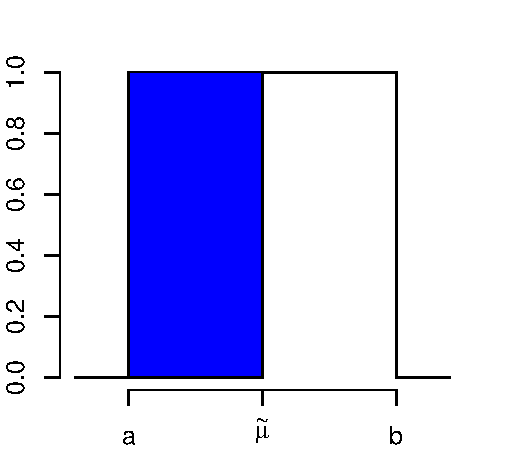
\includegraphics[scale=.5]{ch4_pdf_unif3.pdf}
\end{tabular}

\vspace{.3cm}
\uncover<6->{In this case, the median $\tilde\mu$ is the same as the mean $\mu$.}
\end{frame}

\begin{frame}{Median of a Exponential Random Variable}
\begin{block}{}
Find the median of an exponential random variable $X$ with rate $\lambda$.
\end{block}
\pause Solution: We need to find $x$ such that $P(X \leq x)=1/2$. \pause Recall
$$P(X \leq x) = F(x) = \int_0^x \lambda e^{-\lambda t}\ dt = 1-e^{-\lambda x}$$

\vspace{-.2cm}
\begin{tabular}{p{4.5cm}p{6cm}}
\vspace{0cm}
\pause We just need to solve
$$\frac12 = 1-e^{-\lambda x}$$
for $x$. \pause This gives $$x=\frac{\ln 2}{\lambda} = \mu\ln 2$$
\pause 
&\vspace{-.4cm}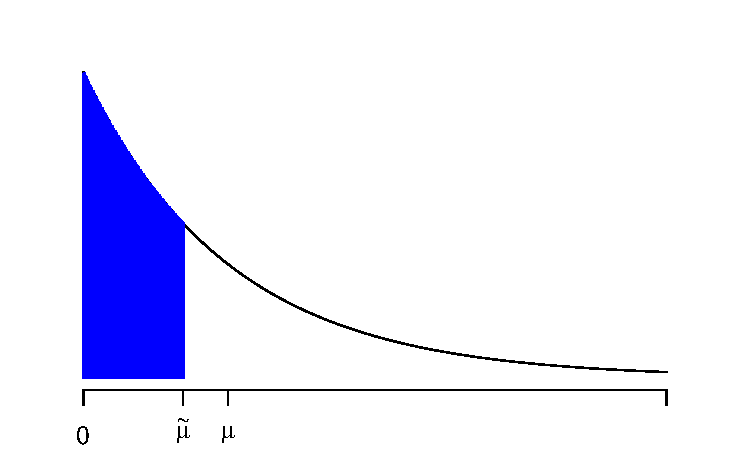
\includegraphics[scale=.55]{ch4_cdf_exp2.pdf}
\end{tabular}

\vspace{-.2cm}
So the median is $\tilde\mu = \mu\ln 2 \approx .693 \mu$.
\end{frame}

\begin{frame}{Percentiles of a Continuous Random Variable}
\begin{block}{}
Given a continuous random variable $X$ and $0\leq p\leq 1$, the $100p$th \emph{percentile} of $X$ is the value $x$ such that $P(X \leq x)=p$.
\end{block}
Note: The \textit{median} is the same thing as the 50th percentile.

\vspace{.2cm}
\pause Example: Find the 90th percentile of a uniform random variable $X$ on [10,40]:
\pause \begin{align*}
.9 = P(X\leq x) = \int_{10}^x \frac1{40-10}\ dt = \frac{x-10}{30}
\end{align*}
\pause Solving for $x$,
$$x=(.9)(30)+10 = 37$$
\pause So the 90th percentile of $X$ is 37.
\end{frame}


\begin{frame}{Problem}
\begin{block}{}
Given a Poisson process with rate $\lambda$, find the pdf of the amount of time $X$ we must wait until $k$ events have occurred.
\end{block}
\pause Let $Y_t$ be the number of events which have occurred by time $t$, so $Y_t$ is a Poisson random variable with mean $\mu=\lambda t$. \pause The cdf of $X$ is
\begin{align*}
F(t)&=P(X \leq t) = P(Y_t \geq k) \\
\uncover<4->{&=1-P(Y_t < k) \\}
\uncover<5->{&=1-\sum_{j=0}^{k-1} \frac{e^{-\mu} \mu^j}{j!}\\}
\uncover<6->{&=1-\sum_{j=0}^{k-1} \frac{e^{-\lambda t} (\lambda t)^j}{j!}}
\end{align*}
\end{frame}

\begin{frame}
Differentiating the cdf, we find the pdf of $X$:
\begin{align*}
f(t) &= F'(t) = \frac{d}{dt}\left[1-\sum_{j=0}^{k-1} \frac{e^{-\lambda t} (\lambda t)^j}{j!}\right]
\uncover<2->{= -\sum_{j=0}^{k-1} \frac{\lambda^j}{j!} \frac{d}{dt}(e^{-\lambda t}t^j) \\}
\uncover<3->{&= -\sum_{j=0}^{k-1}\frac{\lambda^j}{j!}(-\lambda e^{-\lambda t}t^j+e^{-\lambda t}jt^{j-1})\\}
\uncover<4->{&= \sum_{j=0}^{k-1}\frac{\lambda^{j+1}e^{-\lambda t}t^j}{j!} - \sum_{j=1}^{k-1} \frac{\lambda^j e^{-\lambda t}t^{j-1}}{(j-1)!}\\}
\uncover<5->{&= \sum_{j=0}^{k-1}\frac{\lambda^{j+1}e^{-\lambda t}t^j}{j!} - \sum_{j=0}^{k-2} \frac{\lambda^{j+1} e^{-\lambda t}t^j}{j!}}
\uncover<6->{= \frac{\lambda^k e^{-\lambda t}t^{k-1}}{(k-1)!}}
\end{align*}
\end{frame}


\begin{frame}{Gamma Distribution}
\begin{block}{}
Given a Poisson process with rate $\lambda$, the waiting time for $k$ events has a \emph{gamma distribution}, with pdf
$$f(x) =\begin{cases} \frac{\lambda^k}{(k-1)!}x^{k-1}e^{-\lambda x}, & x\geq 0 \\ 0, & x<0\end{cases}$$
\end{block}

\vspace{.2cm}\uncover<3->{ 
When $k=1$ this is an exponential distribution: $f(x) = \lambda e^{-\lambda x}$}

\uncover<2->{
\begin{center}
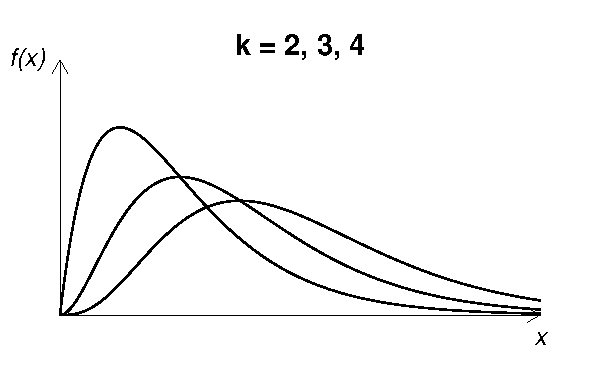
\includegraphics[scale=.7]{ch4_pdf_gam2.pdf}
\end{center}}
\end{frame}

\begin{frame}{Gamma as Sum of Exponentials}
Given a Poisson process with rate $\lambda$, the waiting time for the first event is an exponential random variable $Y_1$ with rate $\lambda$. 

\vspace{.2cm}
\pause
After the first event, the waiting time for the next event is an independent exponential random variable $Y_2$.

\vspace{.2cm}
\pause
Continuing, we see that the waiting time $X$ for $k$ events is the sum of $k$ independent exponential random variables with rate $\lambda$:
$$X=Y_1+\cdots+Y_k$$
\pause In other words, a gamma random variable with parameters $k$ and $\lambda$ may be expressed as a sum of $k$ independent exponential random variables with rate $\lambda$.
\end{frame}

\begin{frame}{Mean and Variance of Gamma Distribution}
Expressing a gamma random variable $X$ as sum of independent exponential random variables allows us to easily calculate the mean and variance of $X$:

\begin{align*}
\uncover<2->{E(X) &= E(Y_1+\cdots+Y_k) \\
&= E(Y_1)+\cdots+E(Y_k) \\
&= 1/\lambda + \cdots + 1/\lambda \\
&= k/\lambda \\[.2cm]}
\uncover<3->{V(X) &= V(Y_1+\cdots+Y_k) \\
&= V(Y_1)+\cdots+V(Y_k) \\
&= 1/\lambda^2 + \cdots + 1/\lambda^2 \\
&= k/\lambda^2}
\end{align*}
\end{frame}



\begin{frame}{Example}
\begin{columns}
\column{6cm}
\begin{block}{}
Cars pass a certain point on a road according to a Poisson process with rate $\lambda=20$ per hour. If we wait until 100 cars have passed, what are the mean and standard deviation of the amount of time we will have to wait? 
\end{block}
\column{4cm}
\includegraphics[width=4.5cm]{road.jpg}
\end{columns}

\vspace{.2cm}
\pause Solution: Let $X$ be the amount of time until 100 cars have passed. $X$ is a gamma random variable with parameters $k=100$ and $\lambda=20$. \pause  We find the mean and standard deviation of $X$ (in hours) using the formulas on the previous slide:
\begin{align*}\mu &= E(X) = k/\lambda = 5\\
\sigma &= \sqrt{V(X)} = \sqrt{k/\lambda^2} = \sqrt{1/4} = 1/2
\end{align*}
%\pause Since $X$ is the sum of 100 iid exponential random variables, the Central Limit Theorem implies that $X$ is approximately normal, so
%\begin{align*}
%P(X > 6) \approx P(Z > 2) \approx .0228
%\end{align*}
\end{frame}

%\begin{frame}{Example}
%\begin{columns}
%\column{6cm}
%\begin{block}{}
%Cars pass a certain point on a road according to a Poisson process with rate $\lambda=20$ per hour. If we wait until 100 cars have passed, what is the probability that we will have to wait more than 6 hours? 
%\end{block}
%\column{4cm}
%\includegraphics[width=4.5cm]{road.jpg}
%\end{columns}
%
%\vspace{.2cm}
%Alternative solution: \pause Let $Y_t$ be the number of cars which have arrived by time $t$ (in hours). $Y_6$ is Poisson with
%\begin{align*}
%\mu&=\lambda t=20\cdot 6 = 120\\
%\sigma&=\sqrt{\mu}=\sqrt{120}\approx 10.95
%\end{align*}
%\pause Since $\mu$ is large, the Central Limit Theorem implies $Y_6$ is approximately normal, so
%$$P(Y_6 < 100) \approx P(Z < -1.83) \approx .0336$$
%\pause (The exact probability is .0279, to 4 decimal places)
%\end{frame}

\begin{frame}{Bernoulli Process vs. Poisson Process}
A sequence of independent Bernoulli random variables $Y_1,Y_2,\dots$ each with parameter $p$ is called a \emph{Bernoulli process} with rate $p$. We interpret this as a process where events occur only at discrete times, 1, 2, 3, \dots, as opposed to a Poisson process where the time of occurence of an event may be any positive real number.

\pause \begin{center}
\begin{tabular}{|p{2.83cm}|l|l|} \hline
& Bernoulli process & Poisson process \\ \hline
\# of events in a unit time period & Bernoulli($p$) & Poisson($\lambda$) \\ \hline
\# of events in a period of length $n$ & Binomial($n,p$) & Poisson($n\lambda$) \\ \hline \hline
Waiting time for first event & Geometric($p$) & Exponential($\lambda$) \\ \hline
Waiting time for $r$ events & Negative Binomial ($r,p$) & Gamma($r,\lambda$) \\ \hline
\end{tabular}
\end{center}
\end{frame}

\begin{frame}{Standard Gamma Distribution}
Recall: the pdf of a gamma random variable with parameters $k$ and $\lambda$ is
$$f(x) =\begin{cases} \frac{\lambda^k}{(k-1)!}x^{k-1}e^{-\lambda x}, & x\geq 0 \\ 0 & x<0\end{cases}$$

\pause A gamma random variable with $\lambda=1$ is called a \emph{standard gamma} random variable. In this case, the pdf becomes
$$f(x) = \begin{cases}\frac1{(k-1)!}x^{k-1}e^{-x}, & x\geq 0 \\ 0, & x<0\end{cases}$$
\pause Since $f(x)$ is a valid pdf, $\int_0^\infty \frac1{(k-1)!}x^{k-1}e^{-x}\ dx = 1$. In other words,
$$\int_0^\infty x^{k-1}e^{-x}\ dx=(k-1)!$$
\end{frame}

\begin{frame}{Gamma Function}
We showed that for any integer $k\geq 1$, 
$$\int_0^\infty x^{k-1}e^{-x}\ dx=(k-1)!$$
\pause In general, this integral exists for any real number $k>0$ and is the definition of the \emph{gamma function} $\Gamma(k)$:
$$\Gamma(k) = \int_0^\infty x^{k-1}e^{-x}\ dx$$
\pause For integers $k\geq 1$, then, $\Gamma(k)=(k-1)!$.
\end{frame}

\begin{frame}{Gamma Function}
$$\Gamma(k) = \int_0^\infty x^{k-1}e^{-x}\ dx$$
\begin{center}
\vspace{-1.5cm}
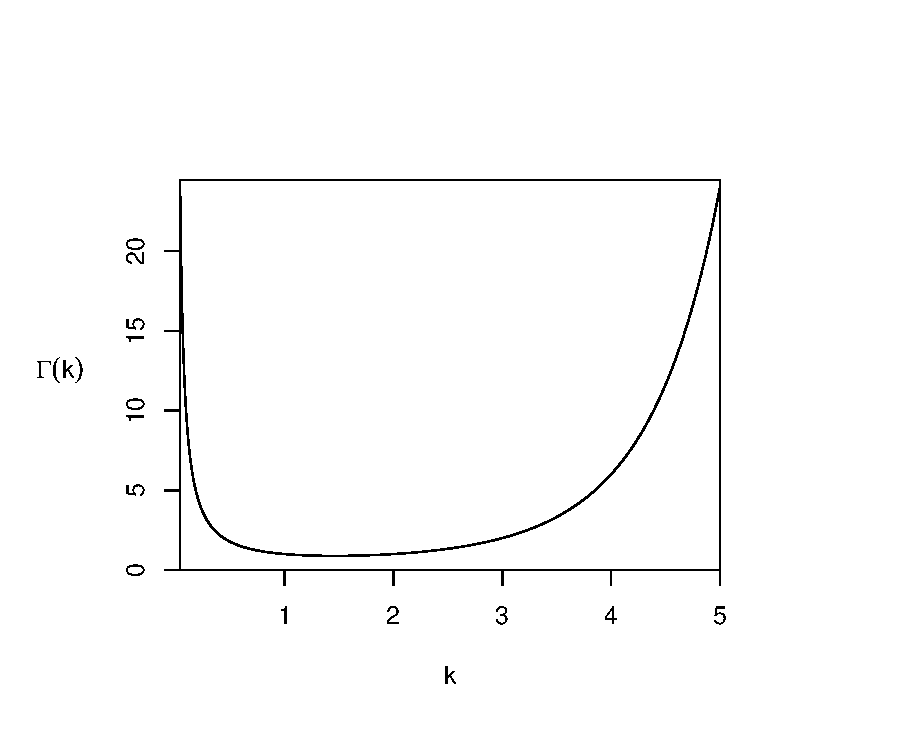
\includegraphics[scale=.7]{ch4_gamfun.pdf}
\end{center}
\end{frame}

\begin{frame}{Gamma Distribution}
Recall: for integer $k\geq 1$, the pdf of a gamma random variable is
$$f(x) =\begin{cases} \frac{\lambda^k}{(k-1)!}x^{k-1}e^{-\lambda x}, & x\geq 0 \\ 0, & x<0\end{cases}$$
\pause Using the gamma function, we may extend the definition of gamma random variables to include cases where $k$ may not be an integer:
\begin{block}{}
A \emph{gamma} random variable $X$ with parameters $k,\lambda>0$ is given by the pdf
$$f(x) = \begin{cases}\frac{\lambda^k}{\Gamma(k)}x^{k-1}e^{-\lambda x}, & x\geq 0 \\ 0, & x<0\end{cases}$$
\end{block}
\end{frame}


%\end{document}
\begin{frame}{Standard Normal Distribution}
\begin{block}{}
We say a random variable $X$ has the \emph{standard normal distribution} if it has pdf
$$\phi(x)=\frac1{\sqrt{2\pi}}e^{-x^2/2}$$
\end{block}
\begin{center}
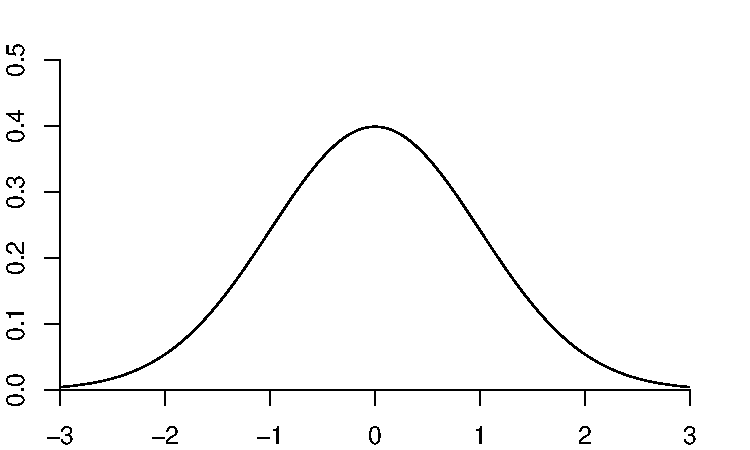
\includegraphics[scale=.5]{ch4_pdf_norm.pdf}
\end{center}
\end{frame}


\begin{frame}{CDF of Standard Normal Distribution}
The cdf of the standard normal distribution is
$$\Phi(x)=\int_{-\infty}^x \frac1{\sqrt{2\pi}}e^{-t^2/2}\ dt$$
There is no simple formula for evaluating this integral. However, it can easily be evaluated numerically by a computer.
\begin{center}
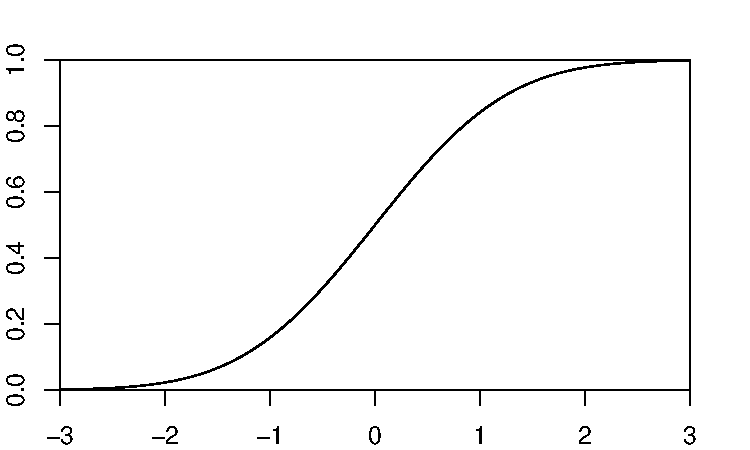
\includegraphics[scale=.5]{ch4_cdf_norm2.pdf}
\end{center}
\end{frame}

\begin{frame}{Standard Normal Distribution}
We want to show that the standard normal pdf is a valid pdf. 
%\begin{align*}
%\uncover<2->{\left(\int_{-\infty}^\infty e^{-x^2}\ dx\right)^2 &= \left(\int_{-\infty}^\infty e^{-x^2}\ dx\right)\left(\int_{-\infty}^\infty e^{-y^2}\ dy\right) \\}
%\uncover<3->{&= \int_{-\infty}^\infty\int_{-\infty}^\infty e^{-(x^2+y^2)}\ dx\ dy\\}
%\uncover<4->{&= \int_0^{2\pi}\int_0^\infty re^{-r^2}\ dr\ d\theta \\}
%\uncover<5->{&= 2\pi \int_0^\infty \frac12e^{-u}\ du = \pi}
%\end{align*}
%\uncover<6->{Therefore $\int_{-\infty}^\infty e^{-x^2}\ dx=\sqrt\pi$, }
%\uncover<7->{so substituting $u=x/\sqrt2$,}
%\begin{align*}
%\uncover<7->{\frac1{\sqrt{2\pi}}\int_{-\infty}^\infty e^{-x^2/2}\ dx
%&= \frac1{\sqrt{\pi}}\int_{-\infty}^\infty e^{-u^2}\ du \\}
%\uncover<8->{&= \frac1{\sqrt{\pi}}\cdot\sqrt{\pi} = 1}
%\end{align*}
%

\pause \vspace{.2cm}
We will use the special integral $\int_{-\infty}^\infty e^{-x^2}\ dx=\sqrt\pi$, which we will prove later. 

\pause \vspace{.2cm}
Assuming this, substituting $u=x/\sqrt2$,
\begin{align*}
\uncover<4->{\int_{-\infty}^\infty \phi(x)\ dx &= \frac1{\sqrt{2\pi}}\int_{-\infty}^\infty e^{-x^2/2}\ dx \\}
\uncover<5->{&= \frac1{\sqrt{\pi}}\int_{-\infty}^\infty e^{-u^2}\ du \\}
\uncover<6->{&= \frac1{\sqrt{\pi}}\cdot\sqrt{\pi} = 1}
\end{align*}

\end{frame}

\begin{frame}{Mean of Standard Normal}
The standard normal distribution is symmetric in the sense that the pdf $\phi(x)$ is an even function, i.e., $\phi(-x)=\phi(x)$:
$$\phi(x)=\frac1{\sqrt{2\pi}}e^{-x^2/2}$$
\pause Therefore the mean of a standard normal random variable is
$$E(X)=\int_{-\infty}^\infty x\phi(x)\ dx =\int_{-\infty}^\infty x\cdot\frac1{\sqrt{2\pi}}e^{-x^2/2}\ dx=0$$
since the integrand is an odd function.
\begin{center}
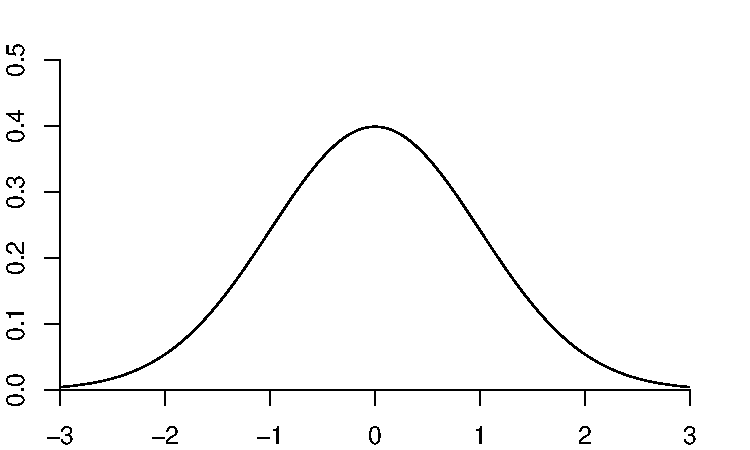
\includegraphics[scale=.5]{ch4_pdf_norm.pdf}
\end{center}
\end{frame}

\begin{frame}{Variance of Standard Normal}
Substituting $u=x^2/2$, note that
\begin{align*}
\int xe^{-x^2/2}\ dx = \int e^{-u}\ du = -e^{-u} = -e^{-x^2/2}
\end{align*}

\pause Integrating by parts,
\begin{align*}
V(X)&=E[(X-\mu)^2] = E(X^2) = \int_{-\infty}^\infty x^2f(x)\ dx \\
\uncover<3->{&= \frac1{\sqrt{2\pi}}\int_{-\infty}^\infty x\cdot xe^{-x^2/2}\ dx \\}
\uncover<4->{&= \frac1{\sqrt{2\pi}}\left[x(-e^{-x^2/2})\big\vert_{-\infty}^\infty + \int_{-\infty}^\infty e^{-x^2/2}\ dx \right] \\}
\uncover<5->{&= \frac1{\sqrt{2\pi}}\int_{-\infty}^\infty e^{-x^2/2}\ dx=1}
\end{align*}
\uncover<6->{\vspace{-.35cm}
\begin{block}{}
A standard normal random variable has mean 0 and variance 1.
\end{block}}
\end{frame}

\begin{frame}{Normal Distributions}
If $Z$ is a standard normal random variable, then given numbers $\mu$ and $\sigma>0$, we can define a new scaled, shifted random variable $X=\sigma Z+\mu$:
\pause\begin{align*}
E(X) &= E(\sigma Z+\mu) = \sigma E(Z)+ E(\mu) = \sigma\cdot 0 +\mu=\mu\\
\uncover<3->{V(X) &= V(\sigma Z+\mu) = V(\sigma Z) = \sigma^2 V(Z) = \sigma^2}
\end{align*}
\uncover<4->{We call $X$ a \emph{normal} random variable with mean $\mu$ and standard deviation $\sigma$, and we write $X \sim N(\mu,\sigma^2)$.
\begin{center}
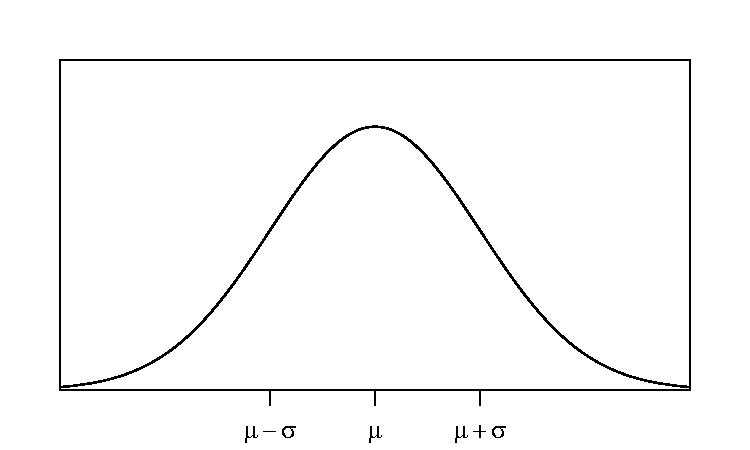
\includegraphics[scale=.5]{ch4_pdf_norm2.pdf}
\end{center}}
\end{frame}

\begin{frame}{CDF and PDF of Normal Distributions}
The cdf of a normal random variable $X\sim N(\mu,\sigma^2)$ is
\begin{align*}
F(x) &= P(X \leq x) = P(\sigma Z+\mu \leq x) \\
\uncover<2->{&= P\left(Z \leq \frac{x-\mu}{\sigma}\right) \\}
\uncover<3->{&= \Phi\left(\frac{x-\mu}{\sigma}\right) }
\uncover<4->{= \int_{-\infty}^{\frac{x-\mu}\sigma} \frac1{\sqrt{2\pi}}e^{-t^2/2}\ dt}
\end{align*}
\uncover<5->{By taking the derivative and applying the chain rule, we find the pdf of $X$:}
\begin{align*}
\uncover<5->{f(x) &= F'(x) }
\uncover<6->{= \frac{d}{dx} \Phi\left(\frac{x-\mu}\sigma\right) \\}
\uncover<7->{&= \frac1\sigma \Phi'\left(\frac{x-\mu}\sigma\right) }
\uncover<8->{= \frac1\sigma \phi\left(\frac{x-\mu}\sigma\right) }
\uncover<9->{= \frac1{\sigma\sqrt{2\pi}}e^{-(\frac{x-\mu}\sigma)^2/2}}
\end{align*}
\end{frame}

\begin{frame}{Example}
\begin{tabular}{@{}p{6cm}@{\hskip .5cm}p{3cm}}
\vspace{0cm}A process produces alginate beads with diameters normally distributed with mean 1 mm and standard deviation .05 mm. Given a random bead, what is the probability that its diameter is between .95 mm and 1.1 mm?
& 
\vspace{0cm}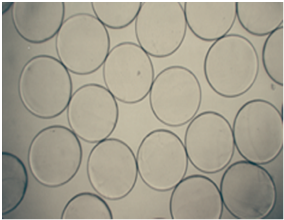
\includegraphics[scale=.5]{alginate.png}
\end{tabular}

\pause \textit{Solution}: The random diameter may be written $X=.05Z+1$, where $Z$ is a standard normal random variable. Then
\begin{align*}
P(.95 \leq X \leq 1.1) &= P(.95 \leq .05Z+1 \leq 1.1) \\
\uncover<3->{&= P\left(\frac{.95-1}{.05} \leq Z \leq \frac{1.1-1}{.05}\right) \\}
\uncover<4->{&= P(-1 \leq Z \leq 2) \\}
\uncover<5->{&= \Phi(2)-\Phi(-1) \approx .9772 - .1587 = .8185}
\end{align*}
\end{frame}

\begin{frame}{Example -- Percentiles}
\begin{tabular}{@{}p{6cm}@{\hskip .5cm}p{3cm}}
\vspace{0cm}A process produces alginate beads with diameters normally distributed with mean 1 mm and standard deviation .05 mm. Find the 90th percentile of bead diameters. 
& 
\vspace{0cm}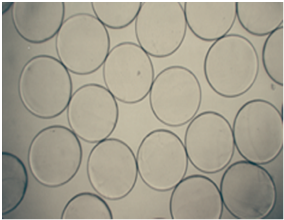
\includegraphics[scale=.5]{alginate.png}
\end{tabular}

\pause \textit{Solution}: As before, the random diameter may be written $X=.05Z+1$, where $Z$ is a standard normal random variable. \pause If $x$ is the 90th percentile, then
 \begin{align*}
.9&=P(X \leq x)=P(.05Z +1 \leq x) \\
\uncover<4->{&= P\left(Z \leq \frac{x-1}{.05}\right) 
\uncover<5->{= \Phi\left(\frac{x-1}{.05}\right)}}
\end{align*}
\uncover<6->{Solving for $x$,}
\begin{align*}
\uncover<6->{x=.05\Phi^{-1}(.9)+1 \approx (.05)(1.28)+1 \approx 1.064\text{ mm}}
\end{align*}
\end{frame}

%\begin{frame}{Symmetry of the Normal Distribution}
%If $Z$ is a standard normal random variable, then $-Z$ is also a standard normal random variable. This symmetry of the standard normal distribution gives rise to some identities:
%\begin{block}{}
%\vspace{-.2cm}
%$$P(Z\geq z) = P(Z\leq -z)$$
%\end{block}
%\begin{center}
%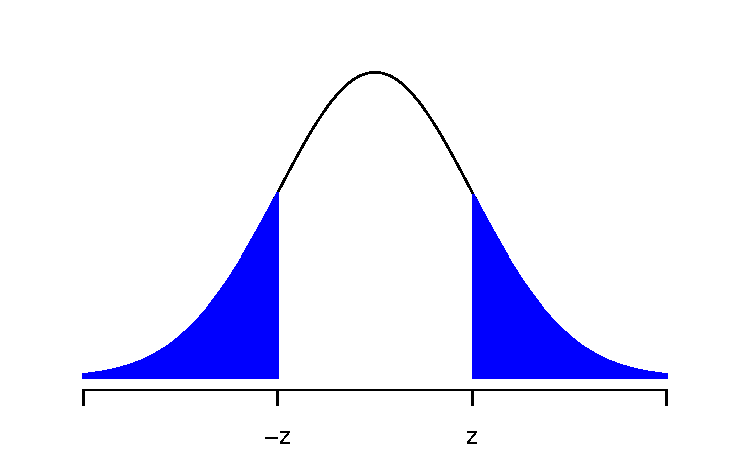
\includegraphics[scale=.5]{ch4_pdf_norm3.pdf}
%\end{center}
%\end{frame}
%
%\begin{frame}{Symmetry of the Normal Distribution}
%Given a symmetric interval $[-z,z]$, the following identity is useful:
%\begin{block}{}
%\vspace{-.2cm}
%$$P(-z \leq Z\leq z) = 1-2P(Z\leq -z)$$
%\end{block}
%\uncover<2->{Proof:} $\begin{aligned}[t]
%\uncover<3->{P(-z \leq Z \leq z) &= 1- P(Z<-z \cup Z>z) \\}
%\uncover<4->{&= 1-(P(Z<-z)+P(Z>z)) \\}
%\uncover<5->{&= 1-(P(Z\leq -z)+P(Z\leq -z)) \\}
%\uncover<6->{&= 1-2P(Z\leq -z)}
%\end{aligned}$
%\begin{center}
%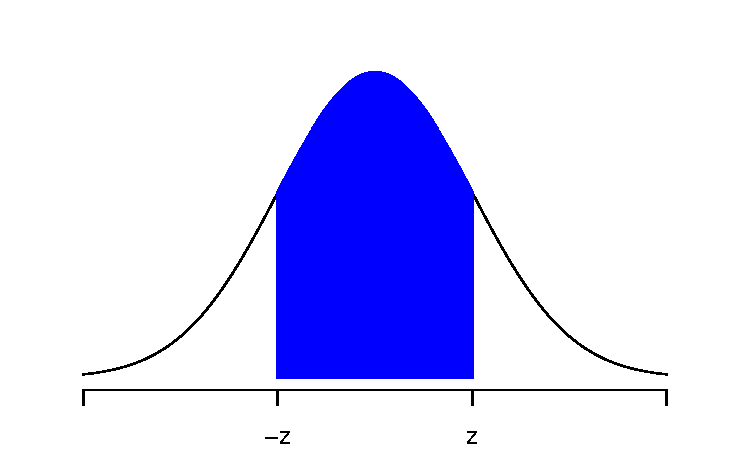
\includegraphics[scale=.5]{ch4_pdf_norm4.pdf}
%\end{center}
%\end{frame}
%
%
%%\begin{block}{}
%%\vspace{-.2cm}
%%$$\Phi(z) = 1-\Phi(-z)$$
%%\end{block}
%%Proof: $\begin{aligned}[t]
%%\Phi(z) &= P(Z \leq z) 
%%= P(-Z \geq -z) \\
%%&= P(Z \geq -z) 
%%= 1-P(Z < -z) = 1-\Phi(-z)
%%\end{aligned}$
%%
%%\begin{block}{}
%%\vspace{-.2cm}
%%$$P(-z \leq Z \leq z) = 1-2\Phi(-z)$$
%%\end{block}
%%Proof: $\begin{aligned}[t]
%%P(-z \leq Z \leq z) &= 1-P(Z<-z \cup Z>z) \\
%%&= 1-(P(Z<-z)+P(Z>z))\\
%%&= 1-(\Phi(-z)+1-P(Z
%%\end{aligned}$
%
%\begin{frame}{Example}
%\begin{block}{}
%If a thermometer reading is normally distributed, with mean $\mu$ equal to the actual temperature, and standard deviation $\sigma$, what value would $\sigma$ have to be to ensure that there is a 95\% chance that the reading is within $\degC{.5}$ of the actual temperature?
%\end{block}
%\pause The reading may be considered as a random variable $X=\sigma Z + \mu$. We want to find $\sigma$ such that
%\begin{align*}
%.95 &= P(\mu-.5 \leq X \leq \mu+.5) \\
%\uncover<3->{&= P(\mu-.5 \leq \sigma Z +\mu \leq \mu+.5) \\}
%\uncover<4->{&= P(-.5/\sigma \leq Z \leq .5/\sigma) \\}
%\uncover<5->{&= 1 - 2P(Z < -.5/\sigma) = 1-2\Phi(-.5/\sigma)}
%\end{align*}
%\uncover<6->{Solving for $\sigma$,
%$$\sigma = -.5/\Phi^{-1}(.025) \approx -.5/-1.96 \approx \degC{.255}$$}
%\end{frame}


%\begin{frame}{Quiz}
%Next class we will have a quiz on normal random variables. 
%
%\vspace{.2cm}
%Bring your standard normal cdf table.
%
%\vspace{.2cm}
%See the Practice Quiz on Canvas.
%
%\begin{center}
%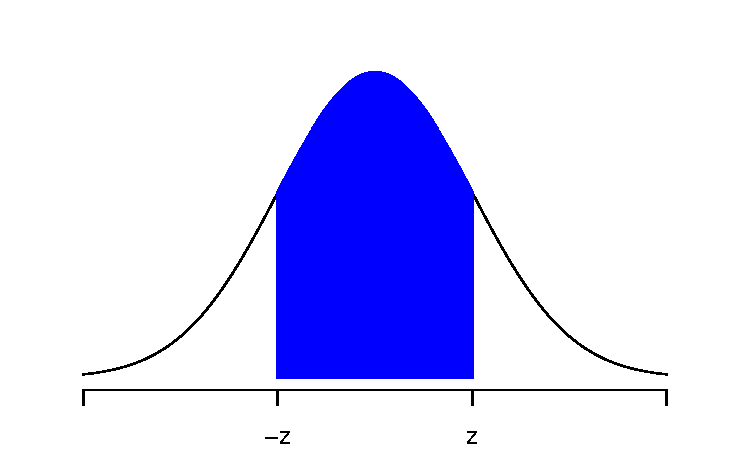
\includegraphics[scale=.5]{ch4_pdf_norm4.pdf}
%\end{center}
%
%\end{frame}


%\begin{frame}{Convergence of Sample Means}
%Suppose we generate a sequence of independent Bernoulli random variables $X_1, X_2, \dots$ with $p=.5$ and take the sample mean $\overline{X}=\frac1n\sum_{i=1}^n X_i$ using  larger and larger sample sizes.
%\begin{center}
%\vspace{0cm}
%\begin{tabular}{p{3.5cm}p{7cm}}
%\vspace{0cm}
%\begin{tabular}{l|l}
%$X_i$ & $\overline{X}$ \\ \hline
%0 & 0 \\
%1 & 1/2 \\
%1 & 2/3 \\
%0 & 2/4 \\
%0 & 2/5 \\
%0 & 2/6 \\
%0 & 2/7 \\
%1 & 3/8 \\
%1 & 4/9 \\
%0 & 4/10
%\end{tabular}
%&
%\vspace{-.2cm}
%\animategraphics[width=6.5cm,height=6.5cm]{6}{ch4_lln_bern}{1}{100}
%\end{tabular}
%\end{center}
%\end{frame}
%
%\begin{frame}{Convergence of Sample Means}
%Let's try doing the same thing using standard uniform random variables.
%
%\begin{center}
%\vspace{0cm}
%\begin{tabular}{p{3.5cm}p{7cm}}
%\vspace{0cm}
%\begin{tabular}{l|l}
%$X_i$ & $\overline{X}$ \\ \hline
%0.771 & 0.771 \\ 
%0.409 & 0.590 \\ 
%0.636 & 0.605 \\ 
%0.291 & 0.527 \\ 
%0.251 & 0.472 \\ 
%0.099 & 0.409 \\ 
%0.922 & 0.483 \\ 
%0.990 & 0.546 \\ 
%0.031 & 0.489 \\ 
%0.113 & 0.451 \\ 
%\end{tabular}
%&
%\vspace{-.2cm}
%\animategraphics[width=6.5cm,height=6.5cm]{6}{ch4_lln}{1}{100}
%\end{tabular}
%\end{center}
%\end{frame}
%
%
%\begin{frame}{Convergence of Sample Means}
%Let's try doing the same thing using exponential random variables with mean $\mu=10$:
%\begin{center}
%\vspace{0cm}
%\begin{tabular}{p{3.5cm}p{7cm}}
%\vspace{0cm}
%\begin{tabular}{l|l}
%$X_i$ & $\overline{X}$ \\ \hline
%11.24 & 11.24 \\ 
%3.73 & 7.49 \\ 
%13.13 & 9.37 \\ 
%0.97 & 7.27 \\ 
%3.19 & 6.46 \\ 
%4.05 & 6.05 \\ 
%12.69 & 7.00 \\ 
%4.11 & 6.64 \\ 
%6.77 & 6.66 \\ 
%7.45 & 6.73 \\ 
%\end{tabular}
%&
%\vspace{-.2cm}
%\animategraphics[width=6.5cm,height=6.5cm]{6}{ch4_lln_exp}{1}{100}
%\end{tabular}
%\end{center}
%\end{frame}
%
%\begin{frame}{Law of Large Numbers}
%A result in probability theory guarantees that this works no matter what the distribution of the $X_i$ is, as long as $E(X_i)$ exists. For instance, the $X_i$ could be Bernoulli, geometric, normal, hypergeometric, binomial, or just about anything else we could imagine. 
%\begin{block}{Law of Large Numbers}
%Let $X_1,X_2,\dots$ be independent, identically distributed (iid) random variables with mean $\mu$. Then as $n\to\infty$, the sample mean $\overline{X}$ converges to $\mu$ with probability 1.
%\end{block}
%\end{frame}
%
%\begin{frame}{Sample Mean of iid Random Variables}
%Let $X_1,\dots, X_n$ be independent, identically distributed (iid) random variables with mean $\mu$ and variance $\sigma^2$. Let $\overline{X}$ be the sample mean 
%$$\overline{X}=\frac1n\sum_{i=1}^n X_i = \frac1n(X_1+\cdots+X_n)$$
%
%\pause\vspace{-.1cm} We can compute the expected value and variance of $\overline{X}$:
%\begin{align*}
%E(\overline{X}) &= E\left(\frac1n\sum_{i=1}^n X_i\right)
%\uncover<3->{= \frac1n \sum_{i=1}^n E(X_i)}
%\uncover<4->{= \frac1n \sum_{i=1}^n \mu }
%\uncover<5->{= \frac1n(n\mu) }
%\uncover<6->{= \mu\\[.1cm]}
%\uncover<7->{V(\overline{X}) &= V\left(\frac1n\sum_{i=1}^n X_i\right) }
%\uncover<8->{= \frac1{n^2} \sum_{i=1}^n V(X_i) }
%\uncover<9->{= \frac1{n^2}\sum_{i=1}^n \sigma^2 }
%\uncover<10->{= \frac1{n^2}(n\sigma^2) }
%\uncover<11->{= \frac{\sigma^2}n}
%\end{align*}
%\uncover<12->{So the expected value of the sample mean $\overline{X}$ is $\mu$, the same as the expected value of each summand. However, the standard deviation $\sigma/\sqrt{n}$ of $\overline{X}$ decreases as we increase the sample size $n$.}
%\end{frame}
%
%
%\begin{frame}{Histogram of Sample Means}
%\hspace*{-.3cm}\begin{tabular}{@{}p{5cm}p{7cm}}
%\vspace{0cm}
%Simulate a standard uniform random variable 20000 times and draw the histogram.
%
%\vspace{.2cm}
%\pause Now simulate standard uniform random variables $X_1$ and $X_2$ and compute the sample mean $\overline{X}=\frac12(X_1+X_2)$; do this 20000 times and draw the histogram.
%
%\pause \vspace{.2cm}
%Now repeat this using larger sample sizes: draw the histogram of 20000 simulations of $\overline{X}=\frac1n(X_1+\cdots+X_n)$, for $n=1,2,3,\dots,10$.
%
%\pause\vspace{.2cm}
%The histogram appears to approach a normal distribution.
% &
%\vspace{0cm}
%\animategraphics[width=7cm,height=7cm,controls]{2}{ch4_clt_unif_hist}{1}{10}
%\end{tabular}
%\end{frame}
%
%\begin{frame}{Histogram of Sample Means}
%Now repeat this but instead of simulating standard uniform random variables, use exponential random variables with $\mu=1$:
%
%\begin{center}
%\animategraphics[width=9cm,height=6cm,controls]{2}{ch4_clt_exp_hist}{1}{10}
%\end{center}
%\end{frame}
%
%\begin{frame}{Central Limit Theorem}
%A powerful result of probability theory guarantees that in general, if $n$ is large, then the sample mean $\overline{X}$ is approximately normal: 
%%with mean $\mu$ and standard deviation $\sigma/\sqrt{n}$.
%\begin{block}{}
%Let $X_1,X_2,\dots$ be independent, identically distributed (iid) random variables with mean $\mu$ and standard deviation $\sigma$. Then
%$$\lim_{n\to\infty} P\left(a \leq \frac{\overline{X}-\mu}{\sigma/\sqrt{n}} \leq b\right) = P(a \leq Z\leq b)=\Phi(b)-\Phi(a)$$
%where $Z$ is a standard normal random variable.
%\end{block}
%\end{frame}
%
%\begin{frame}{Distribution of Sample Means}
%Compare the pdf of a the sample mean $\overline{X}$ of standard uniform random variables with the pdf of a normal random variable as specified in the Central Limit Theorem:
%\animategraphics[width=10cm,height=6cm,controls]{2}{ch4_clt_unif}{1}{10}
%\end{frame}
%
%\begin{frame}{Distribution of Sample Means}
%Compare the pdf of a the sample mean $\overline{X}$ of exponential random variables (with $\mu=10$) with the pdf of a normal random variable as specified in the Central Limit Theorem:
%\animategraphics[width=10cm,height=6cm,controls]{2}{ch4_clt_exp}{1}{30}
%\end{frame}
%
%\begin{frame}{Sums of Random Variables}
%Given iid random variables $X_1,\dots, X_n$  with mean $\mu$ and standard deviation $\sigma$, the Central Limit Theorem tells us that if $n$ is large, then the sample mean $\overline{X}=\frac1n(X_1+\cdots+X_n)$ is approximately normal.
%% with mean $\mu$ and standard deviation $\sigma/\sqrt{n}$.
%
%\vspace{.2cm}\pause
%It follows that the sum $X_1+\cdots+X_n$ is also approximately normal, since the sum is the same as $\overline{X}$ scaled by a factor of $n$.
%% but with mean $n\mu$ and standard deviation $n\cdot\sigma/\sqrt{n} = \sigma\sqrt{n}$.
%
%\vspace{.2cm}\pause 
%Examples:
%\begin{itemize}
%\pause\item A binomial is a sum of iid Bernoulli random variables.
%\pause\item A negative binomial is a sum of iid geometric random variables.
%\pause\item A Poisson$(\mu)$ random variable, where $\mu$ is an integer, is a sum of iid Poisson(1) random variables.
%\end{itemize}
%\pause So all of these examples may be approximated as normal if $n$ is large enough.
%\end{frame}
%
%\begin{frame}{Normal Approximation to Binomial}
%Compare the pmf of a binomial random variable (with $p=.4$) to the pdf of the corresponding normal random variable:
%\animategraphics[width=10cm,height=6cm,controls]{3}{ch4_clt_bern}{1}{27}
%\end{frame}
%
%\begin{frame}{Normal Approximation to Poisson}
%Compare the pmf of a Poisson random variable to the pdf of the corresponding normal random variable:
%\animategraphics[width=10cm,height=6cm,controls]{3}{ch4_clt_pois}{1}{18}
%\end{frame}
%
%\begin{frame}{Example}
%\begin{block}{}
%Bob is a candidate for political office in a large city and must take more than half the votes in order to win the election. Suppose a poll finds that 170 of 300 randomly sampled voters favor Bob. Approximate the probability that the poll would find so many voters favoring Bob if the true proportion were only .5.
%\end{block}
%\pause
%Solution: The number $X$ of sampled voters favoring Bob is a hypergeometric random variable; but since the population is large, we may approximate $X$ as binomial, $\Bin(300,.5)$.
%
%\vspace{.2cm}\pause
%The Central Limit Theorem implies that $X$ is approximately normal, with mean
%$\mu = np=150$ and standard deviation $\sigma=\sqrt{np(1-p)}=\sqrt{75}\approx 8.66$.
%\pause
%\begin{align*}
%P(X \geq 170) &\approx P(8.66Z+150 \geq 170) \\
%\uncover<5->{&\approx P(Z \geq 2.31) \\}
%\uncover<6->{&= P(Z\leq -2.31)} 
%\uncover<7->{ = \Phi(-2.31) }
%\uncover<8->{\approx .0104}
%\end{align*}
%\end{frame}
%
%\begin{frame}{Example}
%\begin{block}{}
%A Geiger counter placed next to a certain radioactive specimen clicks an average of 90 times per minute. Over a 10 minute period, approximate the probability that it would click 800 times or less.
%\end{block}
%\pause Solution: The number of clicks $X$ in a 10 minute period has a Poisson distribution with mean $\mu=900$. The variance of $X$ is $V(X)=\mu=900$, so the standard deviation is $\sigma=\sqrt{900}=30$.
%
%\pause 
%\vspace{.2cm}
%Since $\mu$ is large, the distribution of $X$ is approximately normal. So we can approximate $X$ as $30Z+900$ where $Z$ is a standard normal random variable. \pause Then
%\begin{align*}
%P(X \leq 800) &\approx P(30Z+900 \leq 800) \\
%\uncover<4->{&\approx P(Z \leq -3.33)}
%\uncover<5->{ = \Phi(-3.33) }
%\uncover<6->{\approx .0004 }
%\end{align*}
%\end{frame}
%
%
%\begin{frame}{Problem}
%\begin{columns}
%\column{6cm}
%\begin{block}{}
%A light source emits photons in random directions onto a plane. Find the pdf of the position $X$ at which a random photon hits the plane.
%\end{block}
%\column{4cm}
%\vspace{.1cm}
%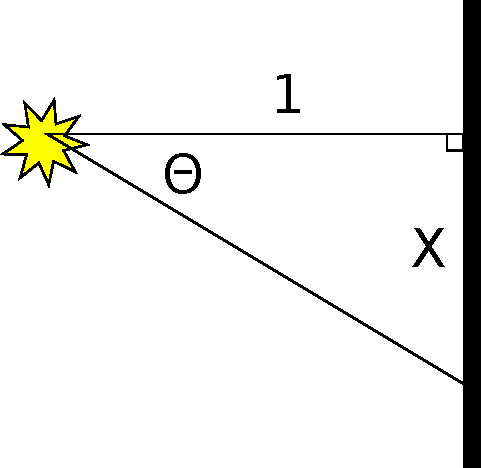
\includegraphics[scale=.35]{light.pdf}
%\end{columns}
%
%\pause Solution: The angle $\Theta$ is uniform on $[-\pi/2,\pi/2]$, so we may write $\Theta=\pi U-\pi/2$ where $U$ is standard uniform. 
%
%\pause \vspace{.1cm}Since $X=\tan \Theta$, we can then calculate the cdf of $X$:
%\begin{align*}
%F(x)&=P(X\leq x)
%\uncover<4->{=P(\tan\Theta \leq x) }
%\uncover<5->{=P(\Theta \leq \tan^{-1}(x)) \\}
%\uncover<6->{&= P(\pi U-\pi/2 \leq \tan^{-1}(x)) }
%\uncover<7->{= P(U \leq 1/2 +\tan^{-1}(x)/\pi) \\}
%\uncover<8->{&= 1/2+\tan^{-1}(x)/\pi}
%\end{align*}
%\uncover<9->{Differentiating, we find the pdf of $X$:}
%\begin{align*}
%\uncover<10->{f(x)=F'(x) = \frac1{\pi(1+x^2)}}
%\end{align*}
%\end{frame}
%
%\begin{frame}{Cauchy Distribution}
%A random variable $X$ has the \emph{standard Cauchy} distribution if it has pdf
%$$f(x)=\frac1{\pi(1+x^2)}$$
%
%\uncover<2->{ \vspace{.1cm}We can check directly that this is a valid pdf: writing $x=\tan\theta$,
%\begin{align*}
%\int_{-\infty}^\infty \frac1{\pi(1+x^2)}\ dx &= \int_{-\pi/2}^{\pi/2} \frac{\sec^2\theta}{\pi(1+\tan^2\theta)}\ dx
%\uncover<3->{=\int_{-\pi/2}^{\pi/2}\frac1{\pi}\ dx}
%\uncover<4->{=1}
%\end{align*}}
%\begin{center}
%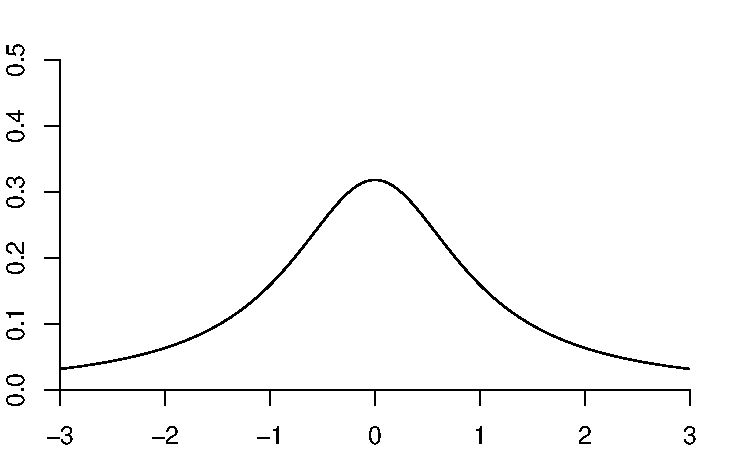
\includegraphics[scale=.5]{ch4_pdf_cauchy.pdf}
%\end{center}
%\end{frame}

%\begin{frame}{Cauchy Distribution}
%To calculate the mean of a standard Cauchy random variable, we find
%\begin{align*}
%\int_0^\infty xf(x)\ dx &= \int_0^\infty \frac{x}{\pi(1+x^2)}\ dx 
%\uncover<2->{ \hspace{1cm} (\text{Setting }u=1+x^2)\\ &= \int_1^\infty \frac1{2\pi u}\ du }
%\uncover<3->{= \frac1{2\pi}\log u\big\vert_1^\infty = \infty \\[.2cm]}
%\uncover<4->{\int_{-\infty}^0 xf(x)\ dx &= \int_{-\infty}^0 \frac{x}{\pi(1+x^2)}\ dx \\}
%\uncover<5->{&= \int_\infty^1 \frac1{2\pi u}\ du }
%\uncover<6->{= \frac1{2\pi}\log u\big\vert_\infty^1 = -\infty}
%\end{align*}
%\uncover<7->{So $E(X)=\infty-\infty$ is undefined. A Cauchy random variable has undefined mean.}
%\end{frame}
%
%\begin{frame}{Divergence of Sample Means}
%Now let's see what happens to the sample mean $\overline{X}$ if we take an iid sequence of Cauchy random variables:
%\begin{center}
%\animategraphics[width=6.5cm,height=6.5cm]{6}{ch4_lln_cauchy}{1}{100}
%\end{center}
%\end{frame}

\begin{frame}{Log-normal Distribution}
\begin{block}{}
A random variable $X$ is said to have a \emph{log-normal} distribution if $\ln(X)$ is a normal random variable.
\end{block}

A log-normal random variable $X$ may be written in the form $X=e^{\sigma  Z+\mu}$, where $Z$ is a standard normal random variable.
\begin{center}
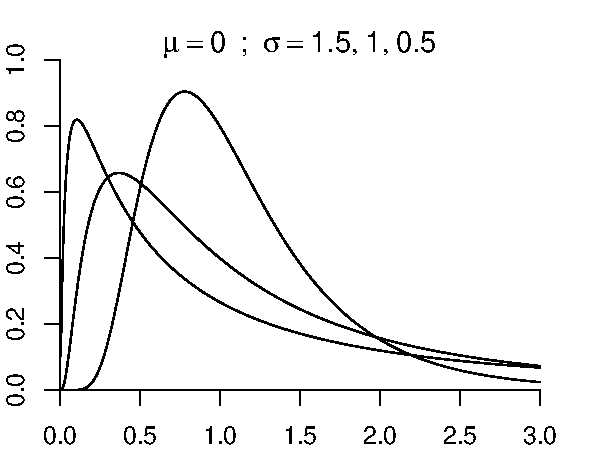
\includegraphics[width=7cm]{ch4_pdf_logn.pdf}
\end{center}
\end{frame}

\begin{frame}{Example}
\begin{columns}
\column{6.5cm}
\vspace{-.2cm}
\begin{block}{}
A certain aerosol spray contains particles whose diameters (in microns) have a log-normal distribution with $\mu=5$, $\sigma=0.5$. What proportion of the particles are larger than 300 microns?
\end{block}
\column{3.5cm}

\includegraphics[width=3.5cm]{aerosol.png}
\end{columns}

\vspace{.2cm}\pause
Solution: The diameter $X$ of a random particle may be written $X=e^{\sigma Z+\mu}$, so
\begin{align*}
P(X > 300) &= P(e^{\sigma Z+\mu} > 300) \\
\uncover<3->{&= P(e^{0.5Z+5} > 300) \\}
\uncover<4->{&= P(Z > (\ln(300)-5)/0.5)\\}
\uncover<5->{&\approx P(Z > 1.41)\\ }
\uncover<6->{&\approx .0793}
\end{align*}
\end{frame}

\begin{frame}{Mean and Variance of Log-normal}
If $X$ is log-normal with parameters $\mu$ and $\sigma$, then
\begin{align*}
E(X) &= e^{\mu+\sigma^2/2}\\
V(X) &= e^{2\mu+\sigma^2}(e^{\sigma^2}-1)
\end{align*}
If $\sigma$ is small, then $X$ is approximately normal:
\begin{center}
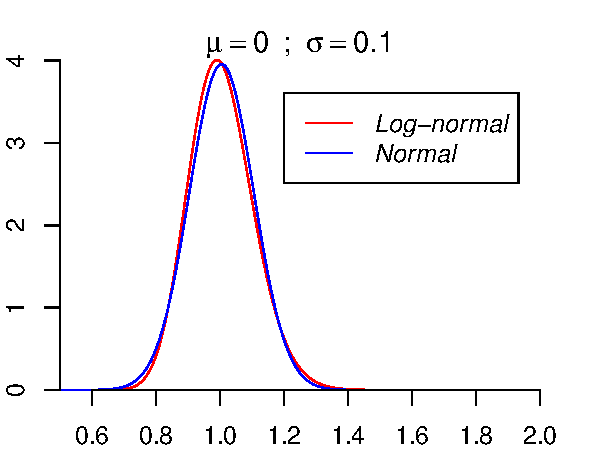
\includegraphics[width=7cm]{ch4_pdf_logn2.pdf}
\end{center}
\end{frame}



%\begin{frame}{Problem}
%\begin{block}{}
%If $Z$ is a standard normal random variable, what is the pdf of $Z^2$?
%\end{block}
%\pause Letting $F(x)$ be the cdf of $X=Z^2$, for $t\geq 0$,
%\begin{align*}
%F(t) = P(Z^2 \leq t) 
%\uncover<3->{&= P(|Z| \leq t^{1/2}) }
%\uncover<4->{= 1-2\Phi(-t^{1/2})}
%\end{align*}
%\uncover<5->{Differentiating, we find the pdf:}
%\begin{align*}
%\uncover<5->{f(t) &= F'(t) = \frac{d}{dt}(1-2\Phi(-t^{1/2})) }
%\uncover<6->{= -2\phi(-t^{1/2})\frac{d}{dt}(-t^{1/2}) \\}
%\uncover<7->{&= t^{-1/2}\phi(t^{-1/2})}
%\uncover<8->{= \frac1{\sqrt{2\pi}}t^{-1/2}e^{-t/2}}
%\end{align*}
%\uncover<9->{Up to a constant factor, we recognize this as the pdf of a gamma random variable, $\frac{\lambda^k}{\Gamma(k)}t^{k-1}e^{-\lambda t}$, with $k=1/2$ and $\lambda=1/2$. }
%\uncover<10->{Since both are valid pdfs, the constant factors must agree; therefore,}
%$$\uncover<10->{\frac1{\sqrt{2\pi}} = \frac{(1/2)^{1/2}}{\Gamma(1/2)} }
%\uncover<11->{= \frac1{\sqrt2\Gamma(1/2)} }
%\uncover<12->{\implies \Gamma(1/2)=\sqrt{\pi}}$$
%\end{frame}

%\begin{frame}{Chi-squared Distribution}
%If $Z$ is a standard normal random variable, then $Z^2$ has a so-called \textit{chi-squared} distribution with one \textit{degree of freedom}. We saw that this is simply a gamma distribution with $k=\lambda=1/2$.
%
%\vspace{.2cm}
%The following generalization has important applications in statistical inference, as we will see later:
%\begin{block}{}
%A \emph{chi-square} random variable with $\nu$ degrees of freedom is a gamma random variable with $k=\nu/2$ and $\lambda=1/2$ and has pdf
%$$f(x) = \begin{cases}\frac1{2^{\nu/2}\Gamma(\nu/2)}x^{\nu/2-1}e^{-x/2},& x\geq 0 \\ 0, & x<0\end{cases}$$
%\end{block}
%\end{frame}

%\begin{frame}{Beta Distribution}
%\begin{block}{}
%A random variable $X$ has a \emph{beta distribution} with parameters $\alpha,\beta>0$ if $X$ has pdf
%$$f(x)=\begin{cases} \frac{\Gamma(\alpha+\beta)}{\Gamma(\alpha)\Gamma(\beta)}x^{\alpha-1}(1-x)^{\beta-1},& 0\leq x\leq 1 \\ 0, & \text{otherwise}\end{cases}$$
%\end{block}
%If $\alpha=\beta=1$, then $X$ is a standard uniform random variable.
%\begin{center}
%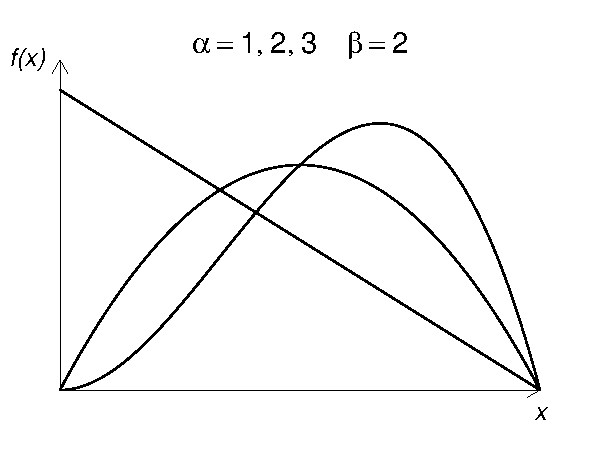
\includegraphics[scale=.5]{ch4_pdf_beta.pdf}
%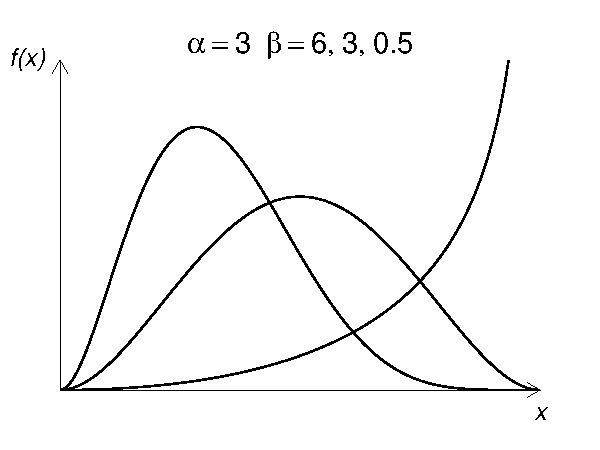
\includegraphics[scale=.5]{ch4_pdf_beta2.pdf}
%\end{center}
%\end{frame}
%
%\begin{frame}{Example}
%\begin{columns}
%\column{6cm}
%\begin{block}{}
%The proportion X of a randomly selected quadrat covered by a plant has a
%beta distribution with $\alpha=4$ and $\beta=3$. What is the probability that a randomly selected quadrat would be less than 40\% covered?
%\end{block}
%\column{3cm}
%\includegraphics[scale=.24]{quadrat.jpg}
%\end{columns}
%
%\vspace{.2cm}
%\pause Solution:
%$\begin{aligned}[t]
%P(X < .4) &= \frac{\Gamma(\alpha+\beta)}{\Gamma(\alpha)\Gamma(\beta)}\int_0^{.4} x^{\alpha-1}(1-x)^{\beta-1}\ dx \\
%\uncover<3->{&= \frac{\Gamma(7)}{\Gamma(3)\Gamma(4)}\int_0^{.4} x^3(1-x)^2\ dx \\}
%\uncover<4->{&= \frac{6!}{2!3!}\int_0^{.4} (x^3-2x^4+x^5)\ dx \\}
%\uncover<5->{&= 60\left(\frac{x^4}4-\frac{2x^5}5+\frac{x^6}6\right)\Big\vert_0^{.4} }
%\uncover<6->{\approx .1792}
%\end{aligned}$
%\end{frame}
%
%\begin{frame}{Mean and Variance of Beta Distribution}
%The mean and variance of a beta distribution are
%\begin{align*}
%\mu &= \frac{\alpha}{\alpha+\beta} \\
%\sigma^2 &= \frac{\alpha\beta}{(\alpha+\beta)^2(\alpha+\beta+1)}
%\end{align*}
%If $\alpha$ and $\beta$ are large, a beta distribution is approximately normal:
%\begin{center}
%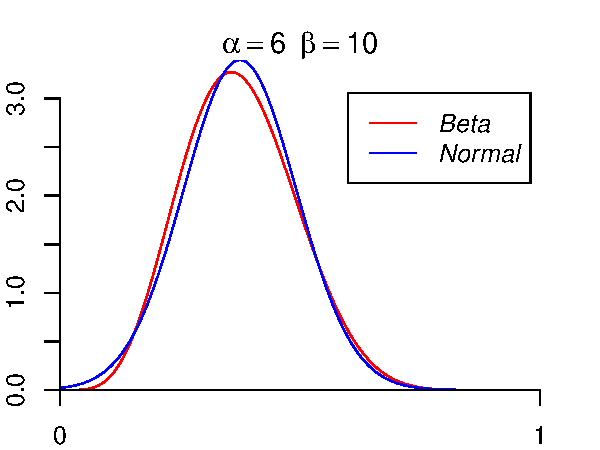
\includegraphics[scale=.6]{ch4_pdf_beta3.pdf}
%\end{center}
%\end{frame}

\begin{frame}{Weibull Distribution}
\begin{block}{}
A \emph{Weibull} random variable $X$ with shape $\alpha>0$ and scale $\beta>0$ has cdf
$$F(x)=\begin{cases}1-e^{-(x/\beta)^\alpha}, & x\geq 0 \\ 0, & x<0\end{cases}$$
Its pdf is
$$f(x)=\begin{cases}\frac{\alpha}{\beta^\alpha}x^{\alpha-1}e^{-(x/\beta)^\alpha}, & x\geq 0 \\ 0, & x<0\end{cases}$$
\end{block}
\begin{center}
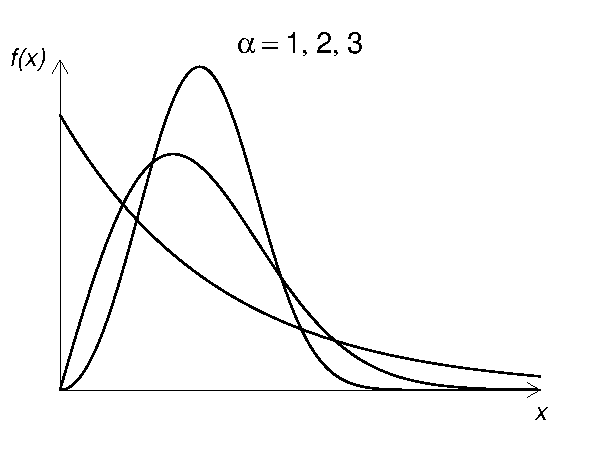
\includegraphics[scale=.5]{ch4_pdf_weibull.pdf}
\end{center}
\end{frame}

\begin{frame}{Example}
\begin{block}{}
The amount $X$ of $\mathrm{NO}_x$ emission (g/gal) from a randomly
selected engine of a certain type may be modeled as a Weibull
random variable with $\alpha=2$ and $\beta=10$. What is the probability that a randomly selected engine has $X \geq 20$?
\end{block}
\pause Solution: The cdf of $X$ is
$$F(x) = P(X \leq x) = 1-e^{-(x/\beta)^\alpha} = 1-e^{-(x/10)^2}$$
\pause Therefore,
\begin{align*}
P(X \geq 20) &= 1-P(X \leq 20) = 1-F(20)\\
&= e^{-(20/10)^2} = e^{-4} \approx .0183
\end{align*}
\end{frame}



\begin{frame}{Summary}
\small
\setlength{\extrarowheight}{.15cm}
\hspace*{-.3cm}
\begin{tabular}{p{2.1cm}|p{3.5cm}|p{1.5cm}|p{2.4cm}}
Distribution & PDF & Mean & Variance\\ \hline
\begin{tabular}{@{}l}Uniform\\[-.2cm] \scriptsize $a \leq x \leq b$\end{tabular} & $\frac1{b-a}$ & $\frac{a+b}2$ & $\frac{(b-a)^2}{12}$\\ \hline
\begin{tabular}{@{}l}Exponential\\[-.2cm] \scriptsize $x \geq 0$\end{tabular} & $\lambda e^{-\lambda x}$ & $1/\lambda$ & $1/\lambda^2$ \\ \hline
\begin{tabular}{@{}l}Gamma\\[-.2cm] \scriptsize $x \geq 0$\end{tabular} & $\frac{\lambda^k}{\Gamma(k)} x^{k-1}e^{-\lambda x}$ & $k/\lambda$ & $k/\lambda^2$ \\ \hline
\begin{tabular}{@{}l}Normal\\[-.2cm] \scriptsize $-\infty < x <\infty$\end{tabular} & $\frac1{\sigma\sqrt{2\pi}}e^{-(\frac{x-\mu}\sigma)^2/2}$ & $\mu$ & $\sigma^2$ \\ \hline
\begin{tabular}{@{}l}Weibull\\[-.2cm] \scriptsize $x \geq 0$\end{tabular} & $\frac{\alpha}{\beta^\alpha}x^{\alpha-1}e^{-(x/\beta)^\alpha}$ & $\beta\Gamma(\frac{\alpha+1}\alpha)$ & $\beta^2\Gamma(\frac{\alpha+2}\alpha)-\mu^2$ \\ \hline
\begin{tabular}{@{}l}Log-normal\\[-.2cm] \scriptsize $x \geq 0$\end{tabular} & $\frac1{x\sigma\sqrt{2\pi}}e^{-(\frac{\ln x-\mu}\sigma)^2/2}$ & $e^{\mu+\sigma^2/2}$ & 
$e^{2\mu+\sigma^2}(e^{\sigma^2}-1)$ \\ \hline
%\begin{tabular}{@{}l}Beta\\[-.2cm] \scriptsize $0 \leq x \leq 1$\end{tabular} & $\frac{\Gamma(\alpha+\beta)}{\Gamma(\alpha)\Gamma(\beta)}x^{\alpha-1}(1-x)^{\beta-1}$ & $\frac\alpha{\alpha+\beta}$ & $\frac{\alpha\beta}{(\alpha+\beta)^2(\alpha+\beta+1)}$
\end{tabular}

\end{frame}

% Central Limit Theorem for Lognormal

% Q Q plot
\end{document}
